%-----------------------------------------------------------------------------
%
%               Template for sigplanconf LaTeX Class
%
% Name:         sigplanconf-template.tex
%
% Purpose:      A template for sigplanconf.cls, which is a LaTeX 2e class
%               file for SIGPLAN conference proceedings.
%
% Guide:        Refer to "Author's Guide to the ACM SIGPLAN Class,"
%               sigplanconf-guide.pdf
%
% Author:       Paul C. Anagnostopoulos
%               Windfall Software
%               978 371-2316
%               paul@windfall.com
%
% Created:      15 February 2005
%
%-----------------------------------------------------------------------------


\documentclass[nocopyrightspace]{sigplanconf}

% The following \documentclass options may be useful:
%
% 10pt          To set in 10-point type instead of 9-point.
% 11pt          To set in 11-point type instead of 9-point.
% authoryear    To obtain author/year citation style instead of numeric.

\usepackage{natbib}
\usepackage{url}
\usepackage[squaren,thinqspace,binary]{SIunits}

\let\fourth\relax               % Undefine a macro
\let\second\relax               % Undefine a macro
\let\degree\relax               % Undefine a macro
\let\cdot\relax                 % Undefine a macro
\usepackage{array}
\usepackage{amsmath}
\usepackage{amssymb}
\usepackage{mathabx}
\usepackage{mathtools}
\usepackage{multirow}
\usepackage{bussproofs}
\usepackage{verbatim}
\usepackage{fancyvrb}

\hyphenation{mono-morph-izing}
\hyphenation{mono-morph-ize}
\hyphenation{mono-morph-ic}
\hyphenation{poly-morph-ic}
\hyphenation{geo-mean}

%------------------------------------------------------------------------------
% Global macro definitions

\newcommand{\abs}[1]{\lvert#1\rvert}
\newcommand{\proportional}{\mathbin{\propto}}
\newcommand{\inst}{\mathrel{\succeq}}
\newcommand{\defeq}{\mathrel{:=}}
\newcommand{\defeqcont}{\mathrel{\hphantom{\defeq}\mathllap{\mid}}}
\newcommand{\overlineX}[1]{\overline{\vphantom{\beta}#1}}
\newcommand{\overlinet}[1]{\overline{\vphantom{t}#1}}
\newcommand{\conexprX}[3]{#1\app\overlineX{#2}\app\overlineX{#3}}
\newcommand{\conexpr}[3]{#1\app\overline{#2}\app\overline{#3}}
\newcommand{\dataexpr}[4]{#1\app\overline{#2}\app\overline{#3}\app\overline{#4}}
\newcommand{\subst}[2]{[#2/#1]}
\newcommand{\substo}[2]{[\overline{#2/#1}]}

\newcommand{\ztype}[1]{\ensuremath{#1_{\text{type}}}}
\newcommand{\name}[1]{\ensuremath{\mathsf{#1}}} % Object functions
\newcommand{\meta}[1]{\ensuremath{\mathrm{#1}}} % Meta-functions
\newcommand{\bmk}[1]{\texttt{#1}}
\newcommand{\app}{\;}

\def\T{\mathbin{::}}

\newcommand{\qforall}[1]{\forall#1.\nolinebreak[1]\:}
\newcommand{\qexists}[1]{\exists#1.\nolinebreak[1]\:}
\newcommand{\qlambda}[1]{\lambda#1 \to}
\newcommand{\qLambda}[1]{\Lambda#1 \to}
\newcommand{\qforallT}[2]{\qforall{#1\T#2}}
\newcommand{\qexistsT}[2]{\qexists{#1\T#2}}
\newcommand{\qlambdaT}[2]{\qlambda{#1\T#2}}
\newcommand{\qLambdaT}[2]{\qLambda{#1\T#2}}

\newcommand{\letE}[1]{\text{\bf let}\;#1\;\text{\bf in}\;}
\newcommand{\letrecE}[1]{\text{\bf letrec}\;#1\;\text{\bf in}\;}
\newcommand{\letfE}[1]{\text{\bf letfun}\;#1\;\text{\bf in}\;}
\newcommand{\caseE}[1]{\text{\bf case}\;#1\nolinebreak[1]\;\text{\bf of}\;}
\newcommand{\dataE}[1]{\text{\bf data}\nolinebreak[1]\;#1\nolinebreak[0]\;\text{\bf where}\;}
\newcommand{\classE}[1]{\text{\bf class}\nolinebreak[1]\;#1\nolinebreak[0]\;\text{\bf where}\;}
\newcommand{\ifE}[3]{\ifO#1\;\thenO#2\;\elseO#3}
\newcommand{\externO}{\text{\bf extern}\;}
\newcommand{\caseO}{\text{\bf case}\;}
\newcommand{\dataO}{\text{\bf data}\;}
\newcommand{\classO}{\text{\bf class}\;}
\newcommand{\ifO}{\text{\bf if}\;}
\newcommand{\thenO}{\text{\bf then}\;}
\newcommand{\elseO}{\text{\bf else}\;}
\newcommand{\whereO}{\text{\bf where}\;}
\newcommand{\ofO}{\text{\bf of}\;}
\newcommand{\letO}{\text{\bf let}\;}
\newcommand{\letrecO}{\text{\bf letrec}\;}
\newcommand{\inO}{\text{\bf in}\;}
\newcommand{\typeO}{\text{\bf type}\;}

\def\kindstar{\ensuremath{\mathord{\star}}}
\def\kindZ{\ensuremath{\mathbb{Z}}}
\def\kindbox{\name{box}}
\def\kindbare{\name{bare}}
\def\kindval{\name{val}}
\def\kindout{\name{mut}}
\def\kindinit{\name{init}}


\def\typeOut{\name{Mut}}
\def\typeStore{\name{Store}}
\def\typeInit{\name{Init}}
\def\typeStored{\name{Stored}}
\def\typeBoxed{\name{Boxed}}
\def\typeAsBox{\name{AsBox}}
\def\typeAsBare{\name{AsBare}}
\def\typeArr{\name{Arr}}
\def\typeRef{\name{Ref}}
\def\typeRep{\name{Rep}}
\def\typeTuple{\name{Tuple}}
\def\typeTupleV{\name{TupleV}}
\def\typeList{\name{List}}
\def\typeInt{\name{Int}}
\def\typeFloat{\name{Float}}
\def\typeBool{\mathbf{2}}
\def\typeMaybe{\name{Maybe}}
\def\typeScatter{\name{Sc}}
\def\typeSz{\name{Sz}}
\def\typeSv{\name{Sv}}
\def\typeZ{\name{Z}}
\def\typePtr{\name{Ptr}}

\def\contuple{\name{tuple}}
\def\constored{\name{stored}}
\def\conboxed{\name{boxed}}
\def\conref{\name{ref}}
\def\conrepr{\name{rep}}
\def\consize{\name{size}}
\def\conasBare{\name{asBare}}
\def\conasBox{\name{asBox}}
\def\concopy{\name{copy}}
\def\conreprInt{\name{repInt}}
\def\conreprTuple{\name{repTuple}}
\def\coniint{\name{z}}
\def\coneiint{\name{exz}}
\def\consz{\name{sz}}
\def\consv{\name{sv}}
\def\conz{\name{z}}
\def\contrue{\name{true}}
\def\confalse{\name{false}}

\newcommand{\Unit}{\langle\mspace{0.75mu}\rangle}
\newcommand{\Prod}[1]{\langle#1\rangle}
\newcommand{\Array}[1]{\mathopen{\text{\sf[}}#1\mathclose{\text{\sf]}}}

\def\iterIdx{\name{Idx}}
\def\iterStep{\name{Step}}
\def\iterFold{\name{Fold}}
\def\iterColl{\name{Coll}}
\def\iterIter{\name{Iter}}

\newcommand{\todo}[1]{\textbf{[#1]}}

\def\proofsep{13pt}

\newcommand{\proofspacing}{%
  \parindent=0cm%
  \everypar={\hskip 0cm plus 1fill}%
  \parfillskip=0cm plus 1fill\relax%
  \parskip=\proofsep}

\newenvironment{inlinecodeexample}%
{\begin{tabbing}}
{\end{tabbing}}

\newcommand{\setwherestretch}{\def\arraystretch{1.15}}
\newcommand{\where}{\hphantom{=\mathord{}}\mathllap{\text{where}}}
\newenvironment{whereblock}[1]%
{\setwherestretch\where\begin{array}[t]{#1}}%
{\end{array}}

%------------------------------------------------------------------------------

\begin{document}

%\titlebanner{banner above paper title}        % These are ignored unless
%\preprintfooter{preprint}   % 'preprint' option specified.

\title{Performance Analysis of Parboil Benchmark using RenderScript}
%\subtitle{}

\authorinfo{Abdul Dakkak \and Cuong Manh Pham \and Prakalp Srivastava}
           {University of Illinois at Urbana-Champaign}
           {\{dakkak, pham9, psrivas2\}@illinois.edu}

\conferenceinfo{CONF 'yy}{Month d--d, 20yy, City, ST, Country} 
\copyrightyear{20yy} 
\copyrightdata{978-1-nnnn-nnnn-n/yy/mm} 
\doi{nnnnnnn.nnnnnnn}

\maketitle

%\category{CR-number}{subcategory}{third-level}

%\terms
%term1, term2

%\keywords
%keyword1, keyword2

\section{Introduction}

Heterogeneous computing promises to address the rising power dissipation problem
of today's traditional homogeneous multi-core
systems. It provides the ability to integrate a variety of processing elements,
such as large and small general purpose cores, GPUs, DSPs, and custom or
semi-custom hardware into a single system. Applications that can efficiently use
the full range of available hardware reap significant energy
savings over conventional processors by executing portions of the code on the
device which optimized for it. This promise of performance along with power efficiency
has led mobile devices such as smartphones
and tablets, which deal with a variety of applications with limited battery
life, to move towards heterogeneous designs.

However, heterogeneity of hardware resources also has led to a diverse landscape
of different programming models, run-time systems, profiling and debugging tools
for application development. The differences are so deep that programmers are
often experts on only one class of device, e.g., an expert GPU programmer will
not have much DSP expertise and vice-versa. This is highly inefficient and
unproductive: we cannot expect applications to use a separate language for each
class of compute unit. If we want applications to use the full range of
available hardware to maximize performance or energy efficiency or both, the
programming environment has to provide common abstractions for available
hardware compute units.

The industry and the research community have been trying to solve this problem.
The recent development of RenderScript~\cite{wiki:RenderScript, RenderScript}
provides a framework for running computationally intensive tasks at a high
performance by using a specialized runtime for parallelizing work across all
processors available on the device, such as multi-core CPUs, GPUs, or DSPs.
RenderScript is therefore removing the burden of load balancing and memory
management from the programmer to the run-time, unlike other solutions such as
OpenCL, where the programmer has more control over the execution semantics of
the application ({\em the programmer decides which part of application would run
on which device and using which part of the memory heirarchy}).  In this fashion
RenderScript is making the computationally intensive part of the application,
that needs to be accelerated on specialized hardware, performance portable
across the various hardware compute units. Also, since the application is not
dependent on the existence and availability of a specific accelerator, the
application is portable across SoCs with varying combinations of compute units.

While such portability is a noble goal, RenderScript achieves it at the cost of
hiding hardware details from the programmer that are critical to good
performance on these accelerator. For example, in GPUs, the placement of data at
various levels of memory hierarchy is critical to good performance.  It is this
reason that most programming languages for GPUs, allow the programmer unlimited
control over memory management. RenderScript too can use GPUs for acceleration,
but completely hides the memory management from the programmer. In the
RenderScript model, application developers only define the part of the
application that needs to be accelerated, and the granularity at which data
needs to be partitioned, while the rest of the responsibilities of memory
management and work distribution among different compute units is handled by
RenderScript compiler and run-time.  This raises an important question of ``how
effective is the RenderScript compiler and run-time?'', which we plan to answer
by doing a comprehensive performance analysis of RenderScript.

Our code is publicly available at \url{https://github.com/cmpham/RSBench}.
Table~\ref{table:parboil} shows the porting status of each version of the
benchmarks in the Parboil Benchmark Suite.


\begin{table}[h]\small
\centering
\begin{tabu}{ | l |[1.5pt] c | c | c | c | c | c |}
    \hline 
    Benchmark & \multicolumn{6}{c|}{Implementations} \\ \cline{2-7}
                      & NC & OMP & J & JT & OCL & RS \\ \tabucline[1.5pt]{-}
    VectorAdd         & C & C   & C    & C      & C      & C \\ \hline
    SGEMM             & C & C   & C    & C      & C      & C \\ \hline
    Stencil           & C & C   & C    & C      & C      & C \\ \hline
    CUTCP             & N & N   & C    & C      & C      & C \\ \hline
    MRI-Q             & N & N   & C    & C      & C      & C \\ \hline
    TPACF             & B & B   & C    & C      & C      & C \\ \hline
    Histogram         & C & B   & C    & C      & C      & C \\ \hline
    BFS               & \multicolumn{6}{c|}{N} \\ \hline
    MRI-G             & \multicolumn{6}{c|}{N} \\ \hline
    SAM               & \multicolumn{6}{c|}{N} \\ \hline
    SPMV              & \multicolumn{6}{c|}{N} \\ \hline
    LBM               & \multicolumn{6}{c|}{N} \\ \hline
    \hline
\end{tabu}
\caption{Parboil Benchmark Porting Status. \textbf{NC} : Native C; \textbf{OMP}
: Native C with OpenMP; \textbf{JT}: Threaded Java; \textbf{OCL} : OpenCL;
\textbf{RS}: RenderScript; \textbf{C}: Completed; \textbf{N} : No
Implementation; \textbf{B} : a bug causes the benchmark to crash.}
\label{table:parboil}
\end{table}



\section*{Overview}

XXX Describe project structure

\section{Parboil Benchmark Framework}

To measure how effective the RenderScript compiler and runtime
    are, we will be porting the Parboil benchmark framework~\cite{Parboil} to
    RenderScript.
The Parboil benchmark framework is a collection
  of 11 compute kernels extracted from
  real world parallel applications.
Initially restricted to CUDA kernels, Parboil is unique in that it offers
  heavily optimized benchmark implementations for different language targets.
The benchmarks have been ported for multicore configurations using C+OpenMP 
  as well as with OpenCL (both optimized an unoptimized).
The 11 kernels are summarized in table~\ref{table:parboil}.

\begin{table}[h]\footnotesize
\centering
\begin{tabular}{ | l | p{4cm} |}
    \hline 
    Benchmark & Description \\ \hline
    Breadth-First Search & Computes the shortest-path of a weighted graph using bread-first search \\
    CUTCP & Computes the Coulomb's potential charge interactions for atoms on a 3D grid \\
    Histogram & Computes a large histogram of a 2D image \\
    Lattice-Boltzmann Method & Simulates a bounded fluid dynamic problem using Lattice-Boltzmann method \\
    Matrix Multiply & Computes the matrix product of two matrices \\
    MRI-Gridding & Computes a grid used in MRI imaging by interpolation \\
    MRI-Q & Computes a calibration matrix used in MRI imaging \\
    Sum of Absolute Differences & Computes the sum of absolute differences common in video encoding algorithms \\
    Spare-Matrix Vector Multiply & Computes the product of a sparse matrix and a dense vector \\
    Stencil & Convolves a Jacobi stencil on a 3D volume \\
    TPACF & Computes the two point angular correlation function for spatial distribution of astronomical bodies \\   
    \hline
\end{tabular}
\caption{Parboil Benchmark Summary}
\label{table:parboil}
\end{table}


\section{Methodology}


\subsection{Performance Analysis}


\subsection{Power Analysis}


Since Android does not offer a way to capture processor usage information
  programatically, we use the Trepn tool by Qualqomm to capture the
  data for us and save it into a {\tt csv} file.   
Trepn, which is limited to Qualcomm based chipsets, reads internal processor
  counters as well as power rail information, both of which are not otherwise
  available programatically.
We set Trepn to read the counters every $100ms$ and measure the load and power
  usage seperatly to decrease the overhead of the profiler.
To reduce overhead, Trepn measure the processor usage information every $100ms$, both
  the frequency and the load are measured sequentially, we therefore need to 
  correct that when parsing the {\tt csv} file.

  
First, we parse each processor reading along with the time stamp for reading
  the file.
Next, we interpolate the measured data (we use linear interpolant) and
  evaluate the interpolant at the application state times (these are the
  times Trepn recieved a signal from our application and correspond to
  timed blocks of code).
We then multiply the load by the frequency, and rescale all the CPU and GPU data (we perform the rescaling on the CPU and GPU seperatly).
Trepn can have measurment errors, resulting in infinite numbers.
To make sure that these do not skew the plots, we clip the range of possible processor reading to be between 1 and the the $0.99$th quantile of the data.
While efforts have been taken to reduce the profiler's overhead, it still 
  ocupies around a $10\%$ overhead.


\section{Related Work}
\label{sec:related}

In term of programming model, RenderScript is similar to OpenCL~\cite{OpenCL}
and CUDA. While CUDA is designed specifically for NVIDIA GPU devices, OpenCL's
goal is similar to RenderScript, which is aiming at simplifying cross-platform
parallel programming for heterogeneous systems.  In fact, Google had an option
to adopt OpenCL, since some Android hardware already has OpenCL
SDKs~\cite{OpenCL:Android}, but they opted to create RenderScript.  Google
justified the choice by arguing that they required not only performance
portability and development efficiency, but also a more intuitive programming
and distribution model.  This decision caused some frustration from the OpenCL
community \cite{androidblockopenCL} and some hardware
vendors~\cite{googlelockin} who had made big investments on OpenCL.

Since being introduced in 2008, OpenCL performance and performance portability
has been extensively evaluated.  The most common of such evaluations is OpenCL's
performance against CUDA on GPUs~\cite{fang2011comprehensive,
weber2011comparing, van2011correlating, vassilev2010comparison,
amorim2009comparing, karimi2010performance, komatsu2010evaluating}.  On
GPUs, OpenCL and CUDA have a similar platform, memory, and programming model,
thus an one-to-one analysis is possible.  Most studies~\cite{weber2011comparing,
van2011correlating, vassilev2010comparison, amorim2009comparing}, from a wide
array of domains, show that CUDA usually achieves better performance (on NVIDIA
GPUs) than OpenCL.  Another consensus among these studies is that OpenCL
provides a sufficient interface for developers to express more architectural
details to improve the performance of their applications.  For example,
studies~\cite{komatsu2010evaluating} and \cite{fang2011comprehensive} show that
most OpenCL kernels can obtain comparable performance with CUDA kernels when
properly optimized.
% In~\cite{shen2012performance}, the authors compare OpenCL
% and OpenMP in the context of application performance on multi-core CPUs using
% the Rodinia benchmark suite~\cite{che2009rodinia}.  From the study, the OpenMP
% implementations generally outperforms the OpenCL ones.  Based on this result,
% the authors picked three OpenCL worse-performed applications, compared the
% performance against OpenMP, and performed manual performance tuning.  Their
% result show that tuned OpenCL applications outperformed the OpenMP in majority
% of the test cases.

According to \cite{komatsu2010evaluating} and \cite{dolbeau2013one}, OpenCL
achieves fairly stable performance across the tested platforms. However, both
studies also illustrate some cases, in which OpenCL does not handle
architectural specifics well, such as memory layout and number of processing
cores. In order to improve the portability of applications, recent OpenCL
versions has an option to let the runtime decides the group size, i.e., the
number of concurrent threads, or wrap size in CUDA's term. However, we are not
aware of any study that evaluates the optimality of this feature.

% Compared with OpenCL, RenderScript's programming model is more restrictive, in
% the sense that it does not let developers to control the execution scheduling,
% i.e., developers do not know whether a particular region of code is going to be
% executed in a CPU or in a GPU at runtime. RenderScript also limits developers
% from expressing architectural specifics, such as the number of processing cores,
% local memory size. This study will evaluate whether hiding architectural details
% results in RenderScript incurring performance loss compared to OpenCL.

There are many recent proposals aiming at making parallel software development
easier and better utilizing multicores and GPUs available in
mobile devices. Chen et al.~\cite{6704508} introduces a new programming model,
called Android-Aparapi, which is based on the Aparapi model~\cite{Aparapi_web}
to allow Android applications to run parallel Java code on GPU via OpenCL.
Qualcomm has been developing an Android programming library and API, called
MARE (Multicore Asynchronous Runtime Environment)~\cite{MARE_qc}, to facilitate writing parallel
C code via Android Native Development Kit (NDK).
Other studies focused on further simplifying the development of RenderScript
code. In order to quickly reuse OpenCL legacy code in Android environments, Yang
et al.~\cite{yang2012o2render} presents a source-to-source translator from
OpenCL to RenderScript. The authors present several challenges of this process,
the most notable one is the differences in the execution models of the two
standards. More recently, Acosta et al.~\cite{alejandro2014performance}
proposes a parallel development framework, called Paralldroid, for improving the
parallelism of programs running in the Android platform. The framework
automatically generates parallel code in C and RenderScript based on
programmers' annotation in Java code. The results show that the auto-generated
RenderScript code often achieves higher performance than the auto-generated
Native C code.

In term of benchmarking RenderScript, study \cite{kemp2013using} compares three
different programming models, namely RenderScript, Remote CUDA (RCUDA), and C++,
of an image processing library in Android platform. The results on a Tegra 3
quad core device evidently show that RenderScript outperforms both the RCUDA and
C++ implementations. Furthermore, this performance gap increases as the size of
the input increases.  However, we are not aware of any work that provides a
systematic evaluation of RenderScript's performance and performance portability.
The only available tool that we might be able to leverage is CompuBench mobile
for RenderScript~\cite{compuBenchMobile}.  But since this benchmark is a
commercial product and does not offer source, we would not be able to perform
thorough analysis using this it.  So in this regard, we will be providing the
first open source benchmark for RenderScript that can be evaluated against
different language paradigms and hadware targets.


\section*{Schedule}

A Gannt chart detailing the duration for each task
  is shown in figure~\ref{fig:schedule}.
In this section we describe the different phases
    of the project.

We have already started the project by looking how
  easy it is to write vector add in Java such that
  it uses the same file format and timing constructs
  as Parboil.
Both vector addition and matrix multiplication have
  already been ported to Java to examine the feasibility
  of the project.
We have also already contacted the RenderScript team
  to understand what resources and services they can
  provide in terms of hardware to aid us in this project.

For the first phase of the project, we plan on porting
  4 of the simplest Parboil benchmarks to RenderScript
  (Matrix Multiply, TPACF, CUTCP, and MRI-Q).
The kernels in these benchmarks are relatively simple, 
  and most of our time would be spent setting up our 
  development environment, refining our workflow and tools, 
  and developing scripts to collect and aggregate the
  performance metrics.
The first phase ends with the first progress report where
    we plan on reporting our results for these benchmarks.


For the second phase of the project, we plan on completing
    our porting process.
There kernels in this phase are more irregular, and thus
    would be more challenging to port.
We suspect these would be the applications where low level
    control and hardware knowledge would benefit performance.
The second phase ends with the second progress report where
    we again will report the results of these benchmarks.


For the last phase of the project, we will finalize the 
    benchmarks and rerun the measurements again.
We will then, time permitting, examine what makes RenderScript
    either efficient or inefficient and what runtime and/or
    compiler optimizations can be performed to either 
    increase performance or increase programmability.
Based on this we will modify our kernels to make use of these
    learned insights and report the performance in the final
    report.

\begin{figure}[t!]
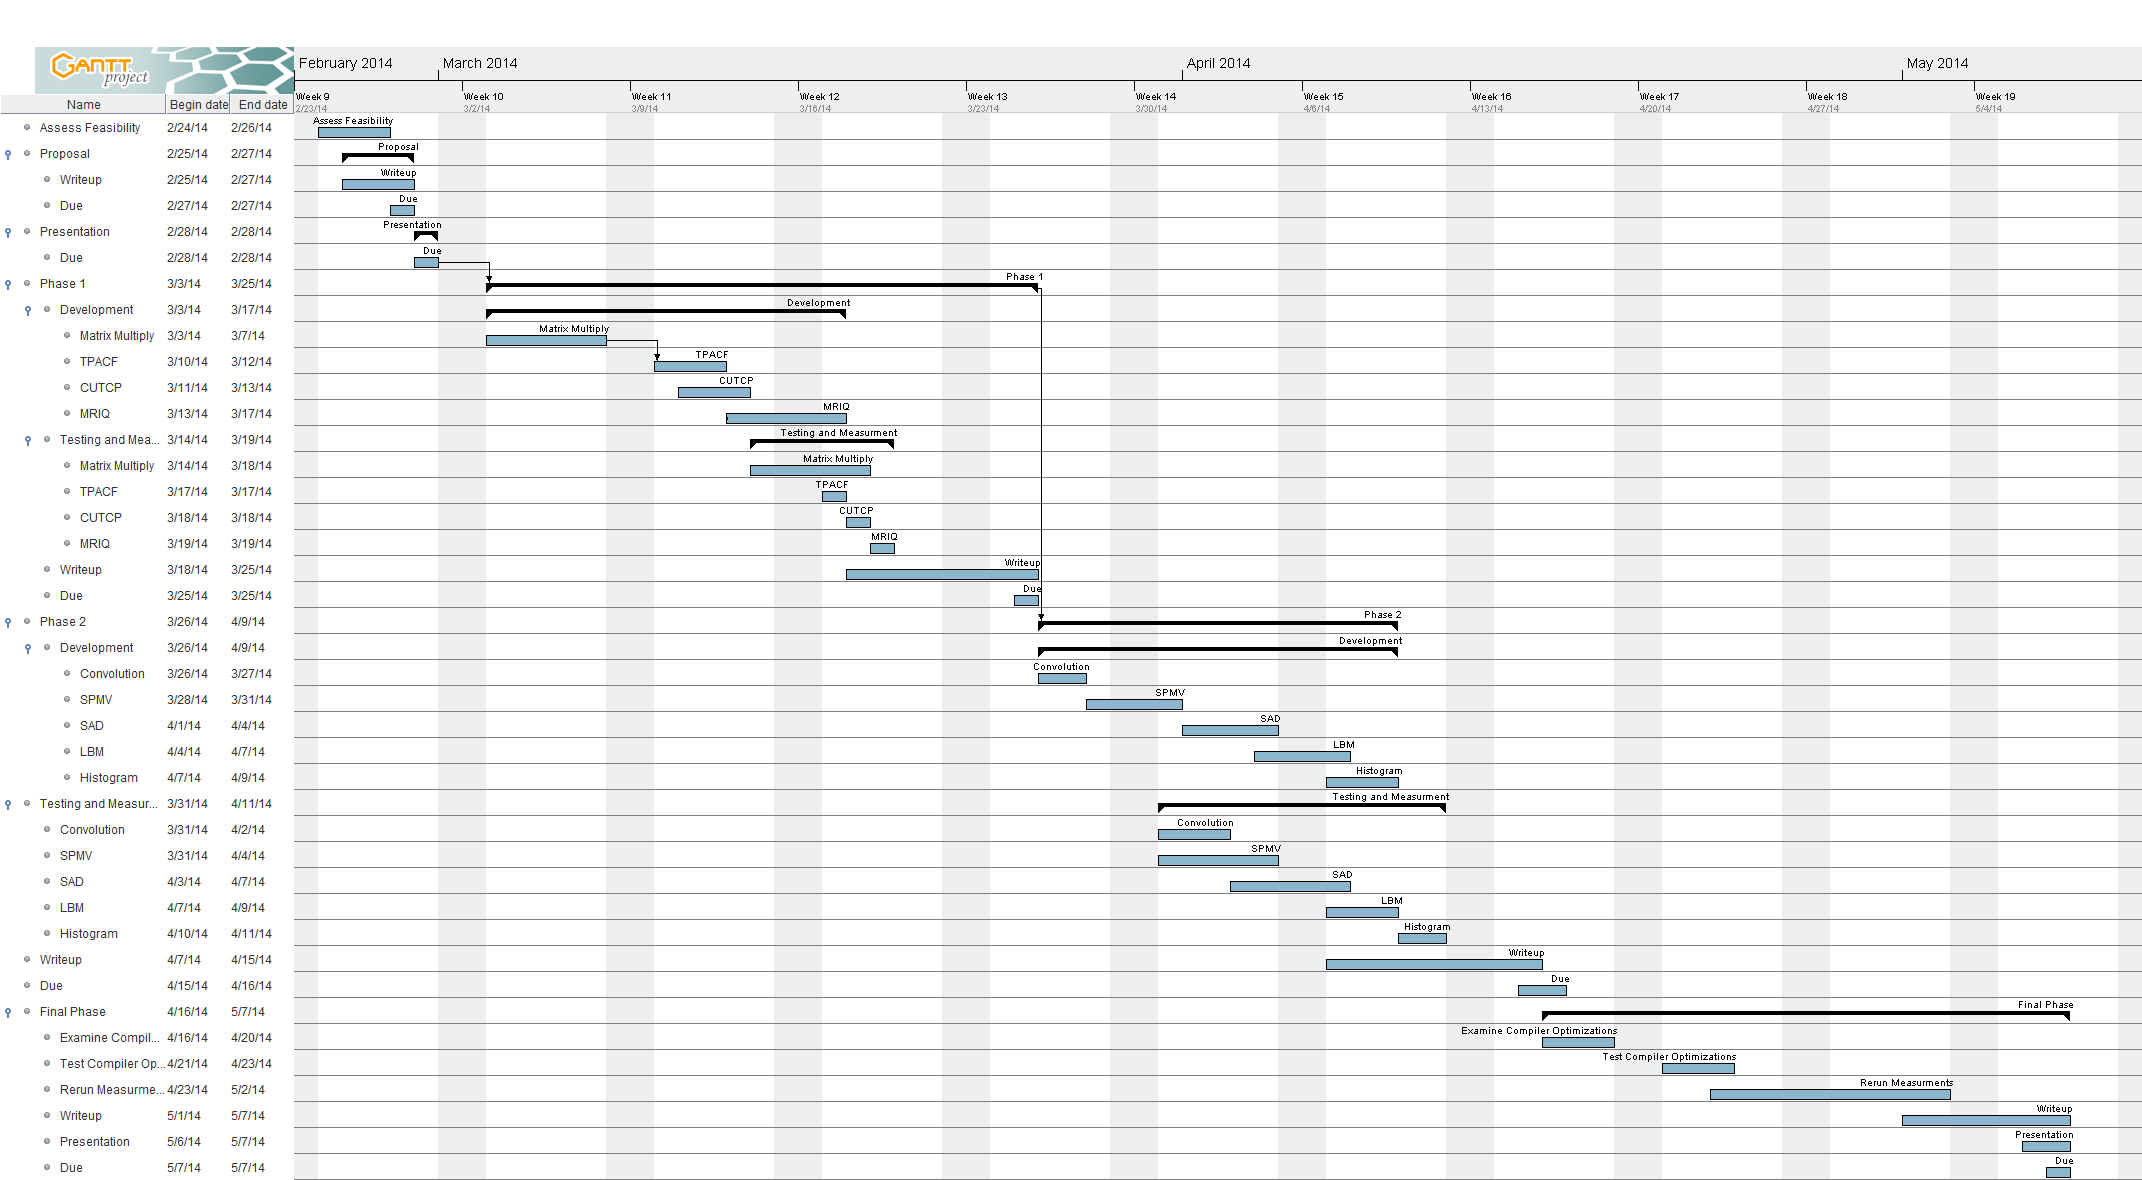
\includegraphics[scale=0.16, angle=90]{chart.png}
\caption{Projected project schedule.}
\label{fig:schedule}
\centering
\end{figure}

\section{Conclusion and Future Work}

RenderScript is awesome?


% We recommend abbrvnat bibliography style.

\bibliographystyle{abbrvnat}
\bibliography{paper}

% The bibliography should be embedded for final submission.

%\begin{thebibliography}{}
%\softraggedright
%
%\bibitem[Smith et~al.(2009)Smith, Jones]{smith02}
%P. Q. Smith, and X. Y. Jones. ...reference text...
%
%\end{thebibliography}

\end{document}
